% sample.tex - rengo.sty 使用例
% 
% 2023-07-14 modified by rengo66 PC
% 2022-07-04 modified by rengo65
% 2021-04-30 modified by rengo64
% 2020-02-26 modified by rengo63 PC
% 2019-07-10 modified by rengo62 PC
% 2006-11-16 modification by TF %SCI07


\documentclass[a4paper]{jarticle}
\usepackage{rengo}
% \usepackage[dvipdfmx]{graphicx}  <- [dvipdfmx]オプションをつけるとエラーになることがあります．
\usepackage{graphicx}
% \usepackage{amsmath}
% \usepackage{amssymb}

\jtitle{
  遺伝的アルゴリズムを用いた2値化畳み込みニューラルネットワークの学習
}
\jauthor{
  ○廣芳大二朗\ \ 内田雅人\ （米子工業高等専門学校）
}
\etitle{
  Training Binary Convolutional Neural Networks Using Genetic Algorithms
}
\eauthor{
  $\ast$T.~Jido, H.~Seigyo (Rengo Univ. ) and J.~Jido (Rengo Corp.)
}
\englishabstract{
  
}
\keyword{

}

\begin{document}

\maketitle

\section{はじめに}

2012年のImageNet Large Scale Visual Recognition Challengeにおいて畳み込みニューラルネットワークを用いた画像認識モデルである
AlexNetが高い認識性能を示したことを受け，ディープラーニングは画像認識をはじめとする様々な分野で利用されるようになった．
一方で，ニューラルネットワークの高性能化に伴い，パラメータ数や計算量が増加し，計算資源やメモリ容量に制約のある環境への適用が課題となっている．
この課題に対する手法として，2015年にCourbariauxらによってBinaryConnectが提案された．
BinaryConnectでは，ニューラルネットワークの重みを-1および+1に二値化することで，メモリ使用量の削減や演算の簡略化を図る．
しかし，二値化関数は微分不可能であるため，通常のバックプロパゲーションをそのまま適用することが困難である．
そこで，勾配計算や関数の微分可能性に依存しない確率的探索手法である遺伝的アルゴリズムに着目する．
本研究では，BinaryConnectを基盤とした二値化ニューラルネットワークに遺伝的アルゴリズムを組み合わせ，勾配計算に依存しない重み最適化手法を提案する．

\section{提案手法}

\subsection{全体の体裁}

A4用紙の（US Letterは不可），縦250 mm，横170 mmの枠内に収まるようにし
てください．
余白は，上20 mm，下27 mm，左20 mm，右20 mmとします．
活字の大きさは，
日本語16ポイント，
日本語著者名・英語タイトル・英語著者名12ポイント，
章タイトル12ポイント，
節タイトル10ポイント，
本文の活字10ポイン
トを目安としてください．
原稿は，
%
\begin{itemize}
  \setlength{\topsep}{0pt}
  \setlength{\partopsep}{0pt}
  \setlength{\itemsep}{0pt}
  \setlength{\parsep}{0pt}
  \setlength{\parskip}{1pt plus 1pt minus 1pt}
  \item 邦文タイトル（英文原稿の場合は不要）
  \item 邦文著者名（登壇者に○印）と著者所属（英文原稿の場合は不要）
  \item 英文タイトル
  \item 英文著者名（登壇者に*印）と英文著者所属
  \item 英文アブストラクト（100ワード程度）
  \item 英文キーワード
  \item 本文，参考文献
\end{itemize}
%
の順に書いてください．
英文キーワードまでを1段組，本文・参考文献を2段組にしてください．

\subsection{図と表}

\begin{figure}[t]
 \centering
 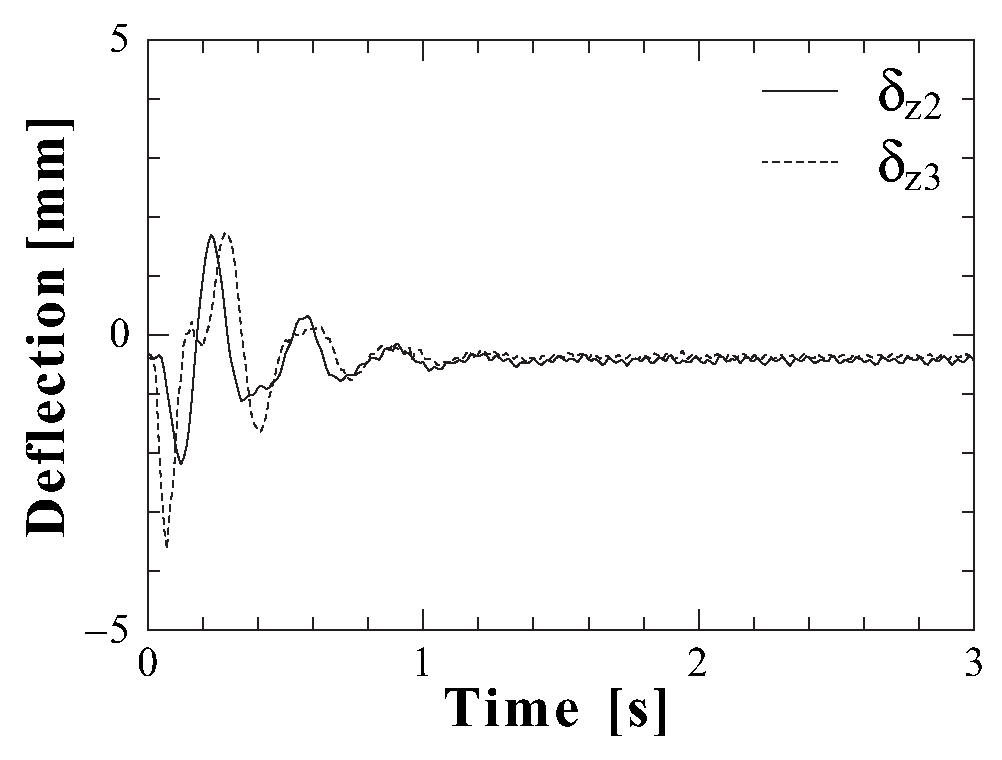
\includegraphics[width=0.8\linewidth]{fig1.eps}
 \caption{A sample figure.  \label{fig:samplefig}}
\end{figure}

図と表は，Fig.~1，Table~1のように番号を振り
（Fig.~\ref{fig:samplefig}\ 参照），図説，図中の説明文は英文で記入してく
ださい．
本文で引用する場合も「Fig.~1に示す」などのようにFig.とTableを使用してく
ださい．

図や表中の文字は小さくなりすぎないよう気をつけてください．
PDF原稿を作成する際，図の画質が劣化しないよう，注意してください．
特にMicrosoft Wordなどで原稿を作成する際，JPEG画像を貼り付けると，一度圧
縮されている画像が再圧縮され画質が劣化するようです．
貼り付ける画像は，画質の良い（圧縮率の低い）画像を用いるか圧縮しない画像
フォーマットを選ぶなど，各自工夫し，最終的なPDFファイルにおいて画質が劣
化しないよう注意してください（300 dpi以上の画質を推奨します）．


\subsection{数式関係}
\verb+eqnarray+ を使うと，等号（とは限りませんが）の両側のスペースが
広くなりすぎるので，この間隔を変更しています．

以下は，\verb+eqnarray+ 環境の使用例です．
\begin{eqnarray}
 \dot{x}(t) & = & A x(t) + B u(t) \\
 y(t) & = & C x(t) + D u(t)
\end{eqnarray}


\subsection{定理環境}
以下は，theorem 環境の使用例です．

\begin{theorem}
ここに定理の内容を記述して下さい．系や補題の場合も同様です．
\end{theorem}
\begin{proof}
ここには定理の証明を記述して下さい．証明の最後には□印がつきま
す．
\end{proof}

定理などの文章は，もともとイタリック書体を使うようになってい
ますが，和文との整合性を考えて，ローマン書体を使うように変更
しています．

\section{参考文献}

文献の引用は本文中に~\cite{web,Conference,Journal}のように書き，
本文の最後にまとめて記述します．次のフォーマットを推奨します．

\begin{enumerate}
  \setlength{\topsep}{0pt}
  \setlength{\partopsep}{0pt}
  \setlength{\itemsep}{0pt}
  \setlength{\parsep}{0pt}
  \setlength{\parskip}{1pt plus 1pt minus 1pt}
	\item[a)] 雑誌論文の場合\\
	$[$番号$]$ 著者：論文題目；雑誌名，Vol.~巻, No.~号, pp.~始ページ--終ページ (発行年)
	\item[b)] 会議論文の場合\\
	$[$番号$]$ 著者：論文題目；会議論文誌名，pp.~始ページ--終ページ (発行年)
	\item[c)] 単行本の場合\\
	$[$番号$]$ 著者：書名，pp.~始ページ--終ページ, 発行所 (発行年)
	\item[c)] Websiteの場合\\
	$[$番号$]$ URL
\end{enumerate}

\begin{thebibliography}{9}
\bibitem{web}
http://www.jjacc.org/

\bibitem{Conference}
自動，制御，自動：
自動制御連合講演会サンプル原稿；
第65回自動制御連合講演会予稿集，pp.~1--4 (2023)

\bibitem{Journal}
T. Jido and J. Jido: Paper title; \textit{Journal Title}, Vol.~1, No.~1, pp.~1--4 (2023)

\bibitem{Book}
H. Seigyo: \textit{Book Title}, pp.~1--4, Publisher (2023)

\end{thebibliography}
\end{document}
% end of template.tex
